In any 3D application we are creating a mathematical model to represent the objects within a given scene. Therefore mathematics plays a very large part in many areas of 3D graphics. Three dimensional mathematics makes use of trigonometry, algebra and even statistics, however in the interest of time, I will be mainly focusing on the specific concepts used in 3D vector, quaternion and matrix mathematics. These concepts contribute to the representation of 3D models as well as model transformations such as: translation, rotation and scaling.  

When representing objects we need to keep track of where they are in the virtual world. In a 2 dimensional world this may be represented by two numbers, an X and a Y position. In 3 dimesions we can represent this with X, Y and Z positions. 3D objects are will usually have a point of origin or global position but in most 3D applications, points or vectors make up triangles. One triangle can be said to be a face and multiple faces will make up a 3D object. In this section we will be looking at the use of points and vectors in 3D graphics.

\section{Points} 

A point is a position in space of $n$-dimensions. In computer graphics applications we usually deal with \acrshort{2d} or \acrshort{3d} coorinate systems. The most common coorinate system used in computer graphics is cartesian coorindates. Cartesian coordinates of a \acrshort{2d} system can be represented by an ordered pair of perpendicular axes, which can be represented as $(p_x, p_y)$. Similarly a point in \acrshort{3d} space can be represented by an ordered triple of perpendicular axes, represended in the form $(p_x, p_y, p_z)$. This can be represented in figure \ref{3DAxisFigure} below.

\begin{figure}[htbp]
	\raggedright
	{\centering
		\vspace{7px}
		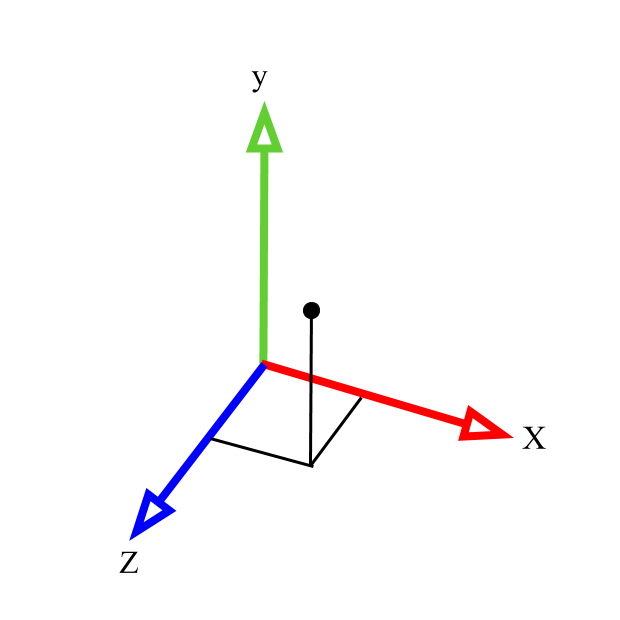
\includegraphics[scale=0.17]{Diagrams/3D_Axis.png}
		\caption{Point in 3D space shown using cartesian coordinates.}
		\label{3DAxisFigure}
	}
\end{figure}
\FloatBarrier

\begin{figure}[htbp]
	\raggedright
	{\centering
		\vspace{7px}
		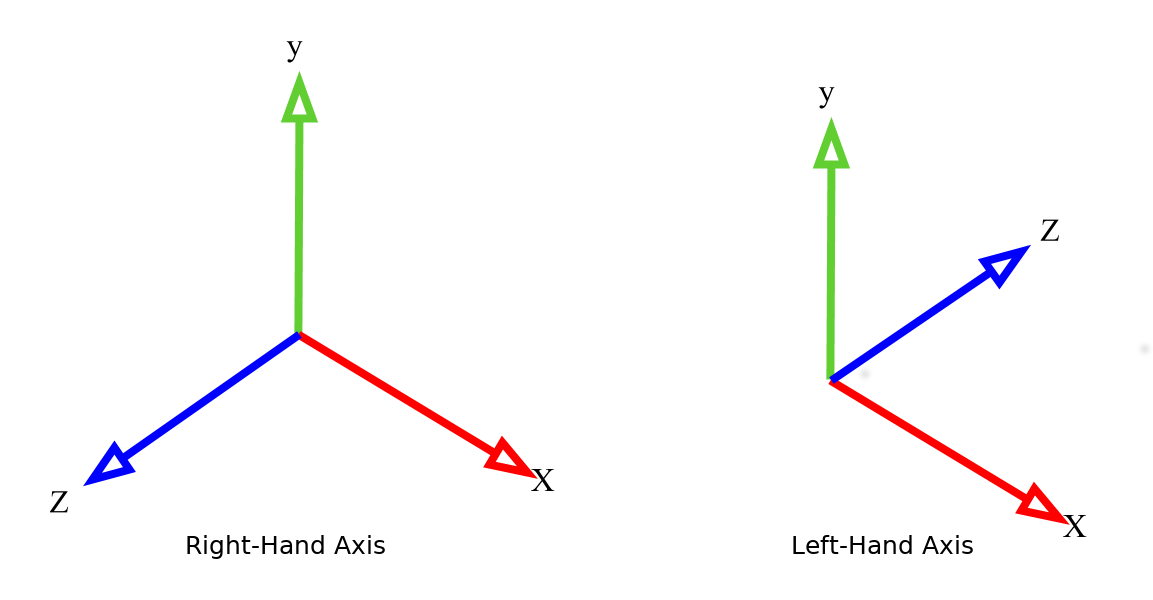
\includegraphics[scale=0.2]{Diagrams/HandAxis.png}
		\caption{Right Hand and Left Hand Coordinate Systems.}
		\label{3DAxisFigure}
	}
\end{figure}
\FloatBarrier

\section{Vector}

Vectors have many meanings in different contexts, In \acrshort{3d} computer graphics, when we talk about vectors we are talking about the Euclidean vector. The Euclidean vector is a quantity in $n$-dimensional space that has both magnitude (the length from A to B) and direction (the direction to get from A to B). \\
Vectors can be represented as a line segment pointing in direction with a certain length. A \acrshort{3d} vector can be written as a triple of scalar values eg: $(x, y, z)$

\begin{figure}[htbp]
	{\centering
		\vspace{7px}
		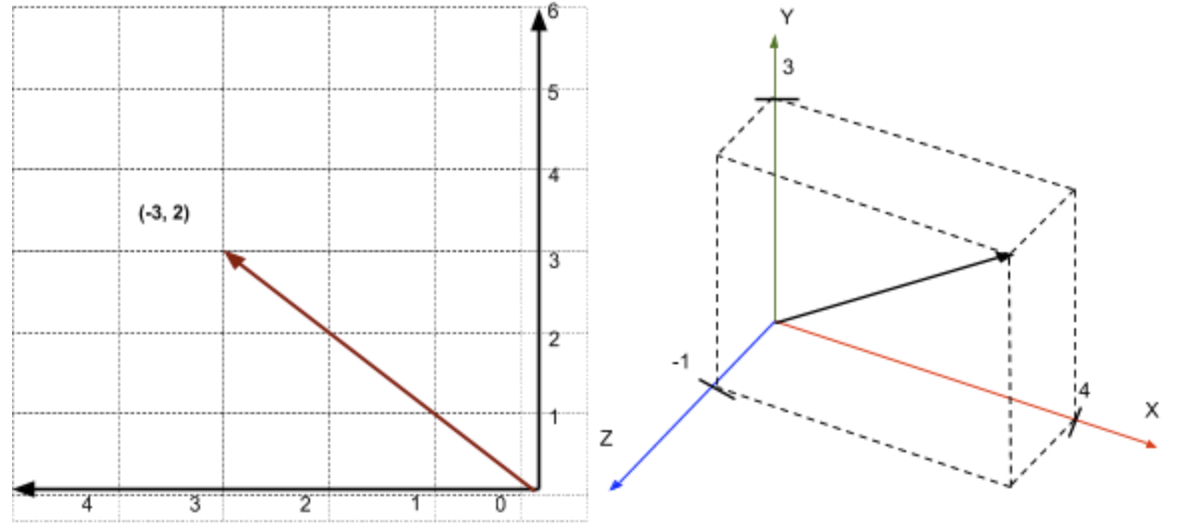
\includegraphics[scale=0.3]{Diagrams/Vector2DAnd3D.png}
		\caption{2D Vector representing the vector at (-3, 2) And 3D Vector (4, 3, -1).}
		\label{3DAxisFigure}
	}
\end{figure}
\FloatBarrier

\subsection{Vector Multiplication}

\subsection{Vector Addition and Subtraction}

\subsection{Dot and Cross Product}

\section{Matrices}


\begin{equation}
\textbf{M} = \begin{bmatrix}
M_{11} & M_{12} & M_{13} \\
M_{21} & M_{22} & M_{23} \\
M_{31} & M_{32} & M_{33}
\end{bmatrix}
\end{equation}
\begin{equation}
\textbf{M} = \begin{bmatrix}
M_{11} & M_{12} & M_{13} & M_{14}\\
M_{21} & M_{22} & M_{23} & M_{24}\\
M_{31} & M_{32} & M_{33} & M_{34}\\
M_{41} & M_{42} & M_{43} & M_{44}
\end{bmatrix}
\end{equation}

\begin{flushleft}
When it comes to matrices in 3D graphics, instead of using a 3 $\times$ 3 matrix we tend use a 4 $\times$ 4 matrix known as an Atomic Transform Matrix. An atomic Transfom matrix is a concatination of four 4 $\times$ 4 matrices: translations, rotations, scale and shear transforms. Resulting in a 4 $\times$ 4 matrix in the following representation: 
\end{flushleft}

\begin{equation}
\textbf{M} = \begin{bmatrix}
RS_{11} & RS_{12} & RS_{13} & 0\\
RS_{21} & RS_{22} & RS_{23} & 0\\
RS_{31} & RS_{32} & RS_{33} & 0\\
T_{1} & T_{2} & T_{3} & 1
\end{bmatrix}
\end{equation}

\begin{flushleft}
Where $RS$ is a 3 $\times$ 3 matrix containing the rotation and scale where the $4^th$ elements are 0. The $T$ elements represent the translation with the 4th element being 1. 
\end{flushleft}

\subsection{Matrix Multiplication}

\begin{equation}
\textbf{AB} = \begin{bmatrix}
A_{11} & A_{12} & A_{13}\\
A_{21} & A_{22} & A_{23}\\
A_{31} & A_{32} & A_{33}
\end{bmatrix}
\times
\begin{bmatrix}
B_{11} & B_{12} & B_{13}\\
B_{21} & B_{22} & B_{23}\\
B_{31} & B_{32} & B_{33}
\end{bmatrix}
\end{equation}
\begin{equation}
= \begin{bmatrix}
A_{row1} \cdot B_{col1} & A_{row1} \cdot B_{col2} & A_{row1} \cdot B_{col3}\\
A_{row2} \cdot B_{col1} & A_{row2} \cdot B_{col2} & A_{row2} \cdot B_{col3}\\
A_{row3} \cdot B_{col1} & A_{row3} \cdot B_{col2} & A_{row3} \cdot B_{col3}
\end{bmatrix}
\end{equation}

\begin{flushleft}
Matrix multiplication is non-commutative, Meaning order matters.
\begin{equation}
AB \neq BA
\end{equation}
\end{flushleft}



\subsection{Translation}



\subsection{Rotation}

\subsection{Scale}


\section{Quaternions}

\begin{flushleft}
We are able to express 3D rotations in the form of a matrix, however in many ways a matrix is not the optimal way of representing a rotation. Matrices are represented by nine floating point values and can be quite expensive to process particularly when doing a vector to matrix multiplication. There are also situations where we would like to smoothly transition from one rotation to another, this is possible using matrices but ican be very complicated. Quaterions are the miraculous answer to all of these difficulties.\\
Quaternions look similar to a 4D vector $ q = [qx, qy, qz, qw]$, and are represented with a real axis ($qw$) and three imaginary axis $qx, qy, qz$.\\
A quaternion can be represented in complex form as follows: $q = (iq_x + jq_y + kq_z + qw)$. \\ 
We will not get into too much detail as to the derivation of quaterions in mathematics however it is important to understand that any unit length quaternion which obays $q_x^2 + q_y^2 + q_z^2 + q_w^2 = 1$ \\ 

\end{flushleft}

\subsection{Unit Quaternion}
Unit quaternions are what are used for rotations, here we can take the angle and the axis of a rotation and convert it to a unit quaternion using the following formula: \\
$q = [qx, qy, qz]$\\
where\\
$q_x = a_x sin \frac{\theta}{2}$\\
$q_y = a_y sin \frac{\theta}{2}$\\
$q_z = a_z sin \frac{\theta}{2}$\\
$q_w = cos \frac{\theta}{2}$\\
The scalar part $q_w$ is the cosine of the half angle, and the vector part $q_x q_y q_z$ is the axis of that rotation, scaled by sine of the half angle of rotation.  

\subsection{Quaternion Multiplication}

\subsection{Conjugate and Inverse}